\begin{comment}


Estrutura

Introdução (contextualização)
Revisão bibliografica ok
	Historica opcional
	Estado da arte ok
Definição/especificação do problema tratado ok
Metodologia ok
Materiais utilizados ok
Aplicação da metodologia à solução do problema ok
Resultados
Discussão dos resultados
Conclusão
Bibliografia
Anexos


no inicio do trabalho: enfatizar a questao do potencial do framework para teste simultaneo e concorrente de multiplas placas.

http://ieeexplore.ieee.org/search/searchresult.jsp?queryText=automated%20inspection%20x-ray&ranges=2004_2017_Year&sortType=desc_p_Publication_Year

http://ieeexplore.ieee.org/xpls/icp.jsp?arnumber=6756131

http://ieeexplore.ieee.org/xpls/icp.jsp?arnumber=7428400
http://ieeexplore.ieee.org/document/7563179/
http://ieeexplore.ieee.org/document/7428398/
http://ieeexplore.ieee.org/document/7859580/
http://ieeexplore.ieee.org/stamp/stamp.jsp?arnumber=7859580


% parte xyz
Nas etapas finais de montagem do produto final é necessário testar a integração da placa eletrônica com o restante do sistema. Importa aqui assegurar o desempenho dinâmico e funcional do sistema, com testes em velocidade de operação nominal para detectar problemas de temporização e a integração com o outros subsistemas do produto. O método mais comum e difundido para detectar problemas nesta etapa é através de testes funcionais e da execução da aplicação final. Nesta etapa é essencial que se tenha um bom diagnóstico do problema para a identificação e reposição do módulo defeituoso.

Mesmo com o produto em operação, as preocupações com teste e diagnóstico não cessam. É de grande interesse do fabricante e do cliente final a detecção de defeitos pós-produção com o produto em campo, assim como o monitoramento da saúde do sistema. Esta etapa é especialmente desafiadora, pois o acesso às ferramentas e instrumentos específicos de teste e diagnóstico é limitado ou até mesmo impossível. Dessa maneira, o desenvolvimento e implementação de ferramentas de auto-teste (BIST), auto-diagnóstico (BISD), e monitoramento são importantes para garantir as qualidades do produto e de operação do sistema.

Fala-se em diagnóstico, pois, muitas vezes, mesmo com testes apontando falhas, a causa raiz do problema pode não ser devidamente identificada. Isso é especialmente problemático quando o sistema está em operação, isso porque uma falha não devidamente tratada provavelmente retornará para a manutenção, gerando mais custos, e impedindo o processo de identificação da falha de fabricação ou projeto que, por sua vez, influencia na qualidade do produto.Este tipo de situação recebe diversos nomes, como \textit{No Failure Found, No Trouble Found, No Defect Found}.


%todo anexar roteiro anterior?

%todo datasheet do power meter nas referencias http://www.ni.com/pdf/products/us/CAT_USB5680.pdf

        \begin{comment}
        
        O padrão UML possui duas categorias de representação de software: Estrutural e Comportamental. Dentro dela temos:
        
            \begin{itemize}
                \item Diagramas Estruturais
                \begin{itemize}
                    \item Diagrama de Classes
                    \item Diagrama de Objetos
                    \item Diagrama de Componentes
                    \item Diagrama de Estrutura Composta
                    \item Diagrama de Instalação ou de Implementação
                    \item Diagrama de pacotes 
                    \item Diagrama de perfil
                \end{itemize}
                \item Diagramas Comportamentais
                \begin{itemize}
                    \item Diagrama de Casos de Uso
                    \item Diagrama de Transição de estados
                    \item Diagrama de Atividade
                    \item Diagrama de Objetos
                    \item Diagrama de Interação
                    \begin{itemize}
                        \item Diagrama de Sequência
                        \item Diagrama de Interatividade
                        \item Diagrama de Colaboração
                        \item Diagrama de Tempo ou Temporal
                    \end{itemize}
                \end{itemize}
            \end{itemize}
        
            Jà foi descrito o funcionamento nuclear de um ator Por sua simplicidade e também pelo seu compo estar descrito em seus ara representar este sistema, a representação será restrita aos diagramas de classe, e transição de estados.
            
            \subsection{Diagrama de estados}
            \subsection{Diagrama de sequências}
        \end{comment}
 \begin{comment}

                 \begin{figure}
                    \centering
                    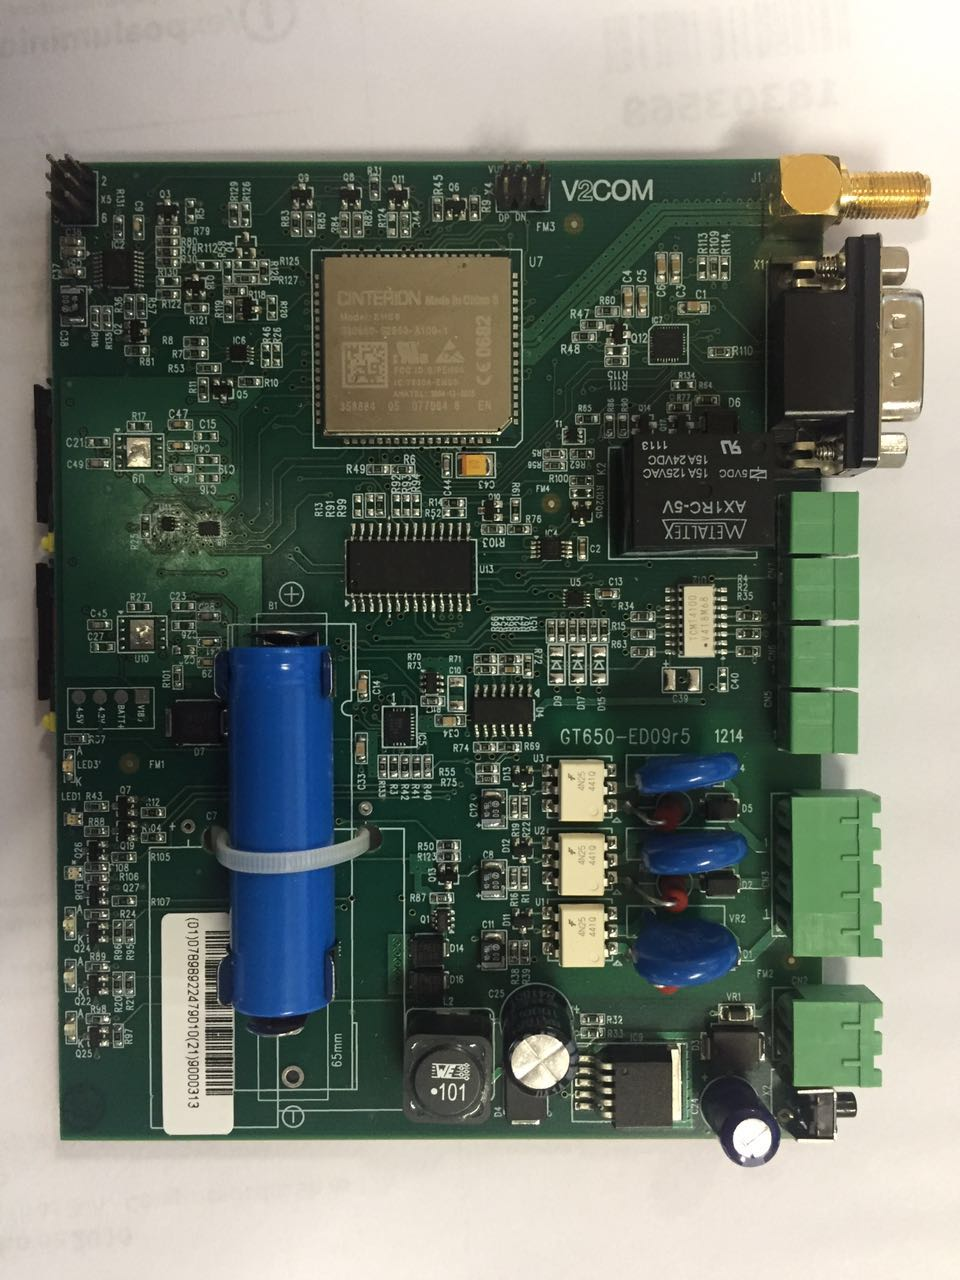
\includegraphics[width=0.9\linewidth]{board}
                    \caption{foto do lado superior  do GT650}
                    \label{fig:board}
                \end{figure}
                
                \begin{figure}
                    \centering
                    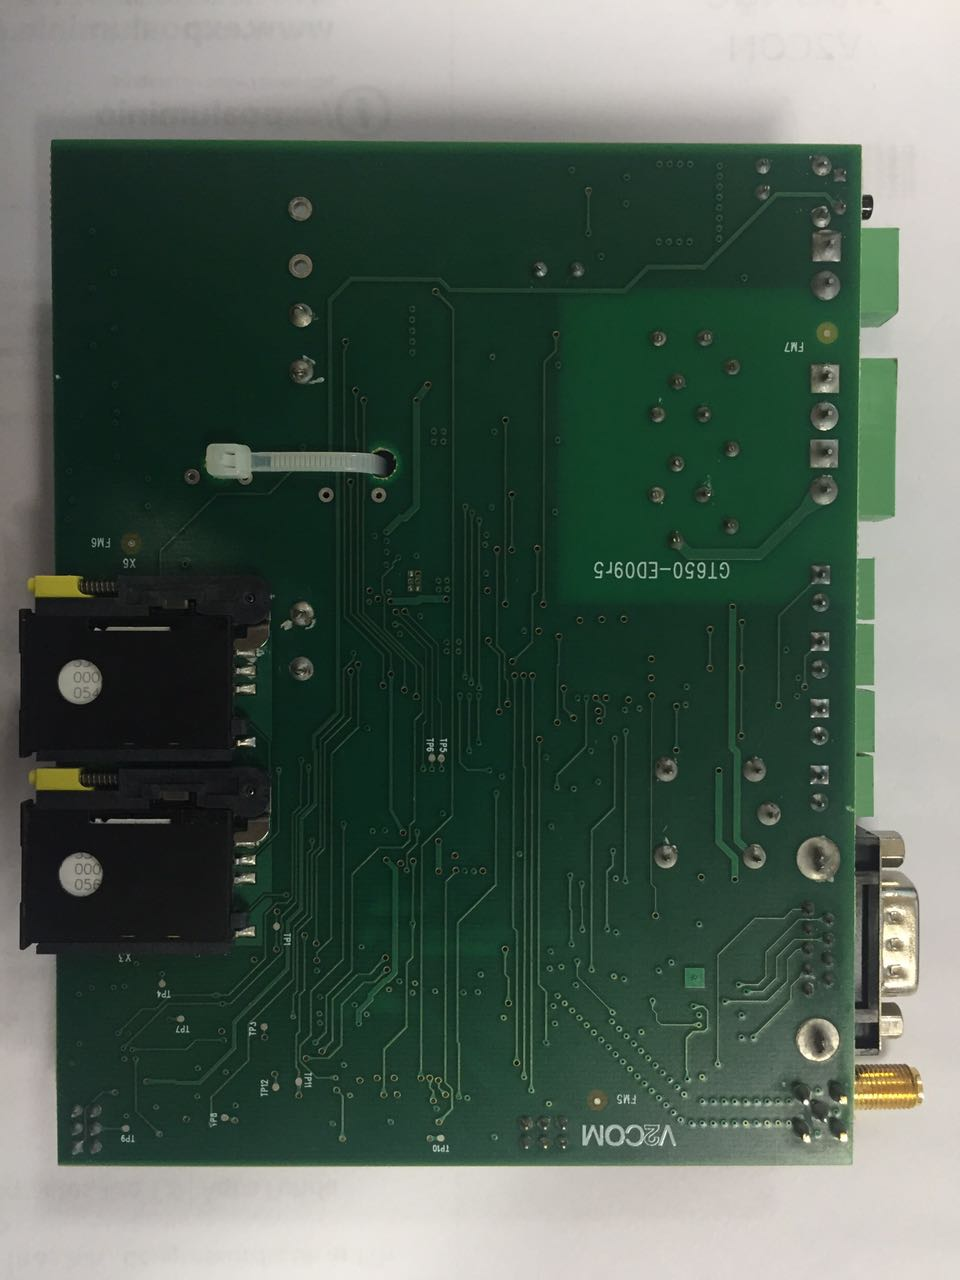
\includegraphics[width=0.9\linewidth]{board_under}
                    \caption{foto do lado inferior  do GT650}
                    \label{fig:board_inf}
                \end{figure}
            \end{comment} 
%https://decibel.ni.com/content/docs/DOC-42227
        
        

http://lup.lub.lu.se/luur/download?func=downloadFile&recordOId=5205504&fileOId=5205517

http://www.iti.uni-stuttgart.de/abteilungen/rechnerarchitektur/projekte/intesys.html

jutman
https://github.com/antonioluppi/TCC/blob/master/references/High%20Quality%20System%20Level%20Test%20and%20Diagnosis%20.pdf


ref q não achei 						
%A. Jutman, "Fighting No Failure Found by Testing Dynamic Faults at Board Level", presented at Emerging Test Strategies - ETS2 of 19th IEEE European Test Symposium (ETS'2014), Paderborn, Germany, May 26-30, 2014
    
    http://www.eng.auburn.edu/~strouce/class/elec6970/NelsonBIST.pdf
    
    http://electronicdesign.com/test-amp-measurement/what-s-difference-between-atpg-and-logic-bist
    
    http://www.design-reuse.com/articles/4430/bist-versus-atpg-separating-myths-from-reality.html
    
    http://wcc.on24.com/event/11/69/47/9/rt/1/documents/slidepdf/1169479_goepel_6216_presentation_final.pdf
    
bug

http://tex.stackexchange.com/questions/54480/package-natbib-error-bibliography-not-compatible-with-author-year-citations
http://tex.stackexchange.com/questions/103664/elsarticle-number-bibliography-not-working

Package natbib Error: Bibliography not compatible with author-year citations. (natbib) Press <return> to continue in numerical citation style. See the natbib package documentation for explanation. Type H <return> for immediate help. ... l.371 ...and\NAT@force@numbers{}\NAT@force@numbers Check the bibliography entries for non-compliant syntax, or select author-year BibTeX style, e.g. plainnat

 
        A partir destes estados, foram levantados os tempos de execução de cada teste que são exibidos na tabela \ref{tab:resultado}. Observa-se pela imagem, uma redução considerável no tempo mínimo e médio de teste. Passando de 
        
        Observa-se que estes resultados foram obtidos somente com a mudança de uma linguagem interpretada para uma compilada, e melhor elaboração do programa, Já que o roteiro é idêntico ao anterior. Certamente que resultados melhores podem ser obtidos se aproveitados os recursos de concorrência de \textit{software} que \textit{framework} oferece. 
        

\end{comment}
